\lstdefinestyle{codeStyleC}{
language=C++,
basicstyle=\ttfamily\normalsize{},
keywordstyle=\color{blue}\ttfamily,
stringstyle=\color{red}\ttfamily,
commentstyle=\color{green}\ttfamily,
breaklines=true,
columns=flexible,
gobble=4,
xleftmargin=\leftmargini,
frame=L,
numbers=left,
numberstyle=\tiny,
belowcaptionskip=0.5em,
belowskip=1em,
}


\chapter{Alternatives to CUDA}
\section{Introduction}
The purpose of this section is to give an overall descriptions and introduction
of the alternative to CUDA. For this work we investigated more in
detail OpenCL and OpenACC. For a full description of all the platform
described here refers to the official documentation.


\section{OpenCL}
Released on December 2008 by the Kronos Group\footnote{A standards
consortium.} OpenCL is an open standard for programming heterogeneous computers
built from CPUs, GPUs and other processors that includes a framework to define
the platform in terms of a host, one or more compute devices, and a
C-based programming language for writing programs for the compute devices (see
figure \ref{openCL}).
One of the first advantages of OpenCL is that it is not restricted to the use of
GPUs but it take each resource in the system as computational peer unit,  easing
the programmer by interfacing with them. Another big advantage is that it is
open and free standard and it permit cross-vendor portability\footnote{One
of the most important supporter of OpenCL is ATI}.
\subsection{Model Architecture}
The model architecture follows that one already studied for
CUDA (see section \ref{cudaProgrammingModel}) but with different names.
\begin{figure}
\centering
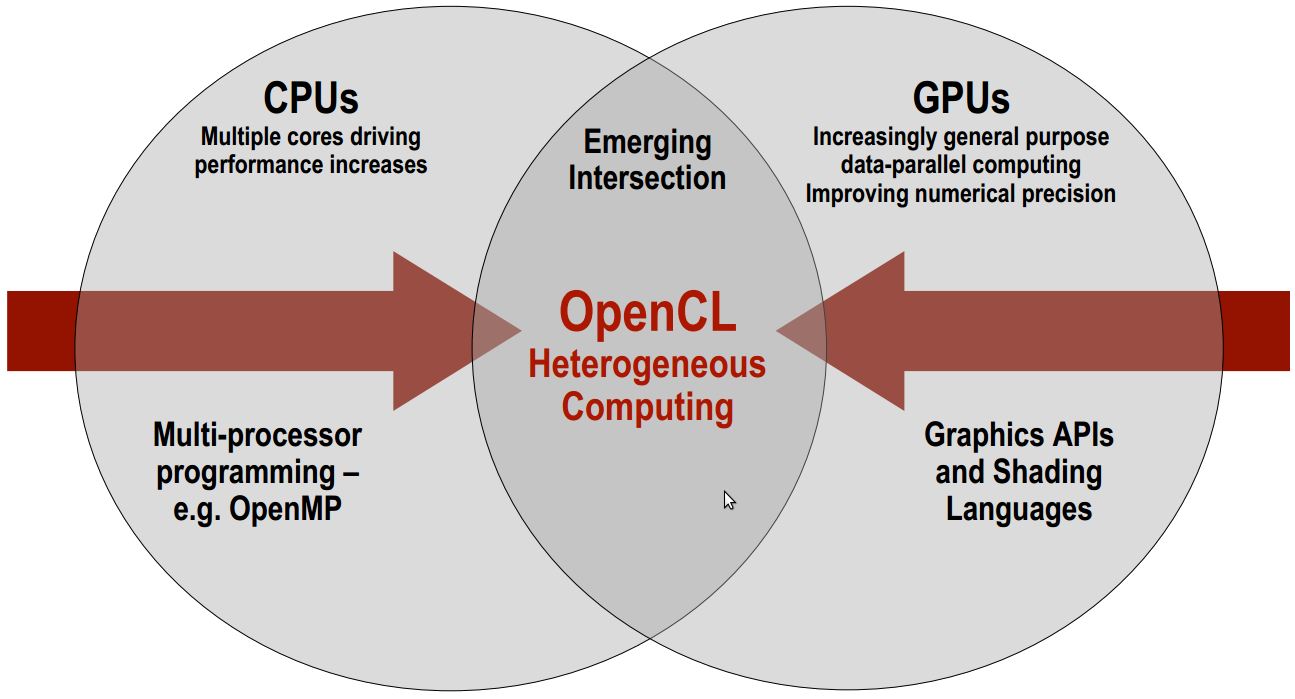
\includegraphics[scale=0.35]{./images/openCL1}
\caption{OpenCL heterogeneous computing.}\label{openCL}
\end{figure}



\begin{description}
  \item [Work-items:] \hfill\\ are equivalent to the CUDA threads and are the smallest execution
entity of the hierarchy. Every time a Kernel is launched, lots of work-items (a
number specified by the programmer) are launched, each one executing the same
code. Each work-item has an ID,  which is accessible from the kernel, and which
is used to distinguish the data to be processed by each work-item.
  \item [Work-group:] \hfill\\  equivalents to CUDA blocks, and their purpose is
  to permit communication between groups of work-items and reflect how the work
  is organized (usually organized as N-dimensional grid of work-groups with
  \begin{math}N \in\{1,2,3\}\end{math}).
  As work-items, they are provided by a unique ID within a kernel.
  Also the memory model is similar to the CUDA's one.
  The host has to orchestrate the memory copy to/from the device and explicit;y
  call the kernel.
\end{description}
  A big difference is in how a kernel is queued to execution on the
  accelerator. Kernels are usually listed in separate
  files the OpenCL runtime take that source code to create kernel object that
  can be first decorated with the parameters on which it is going to
  be executed and then effectively enqueued for execution onto device.
  Here a brief description of the typical flow of an OpenCL application.
  
  \begin{enumerate}
    \item Contexts creation: The first step in every OpenCL application is to
    create a context and associate to it a number of devices, an available
    OpenCL platform (there might be present more than one implementation), and
    then each operation (memory management, kernel compiling and running) is
    performed within \emph{this} context. In the example
    \ref{code:openCLContext} a context associated with the CPU device and the
    first finded platform is created.\\
    
    \item Memory buffers creation: OpenCL buffer Object are created. Those
    buffer are used to hold data to be computed onto devices.\\
    
    \item Load and build program: we need to load and build the compute program
    (the program we intend to run on devices). The purpose of this phase is to
    create an object \textbf{\textit{cl::Program}} that is associable with a
    context and then proceed building for a particular subset of
    context's devices. We first query the runtime for the available devices and
    then load directly source code as string in a
    \textbf{\textit{cl::Program:Source}} OpenCL object (see listing1
    \ref{code:loadBuildProgramCL}).\\

\item In order a kernel to be executed a \emph{kernel object} must be created.
	For a given \emph{Program} there would exists more than one entry point
	(identified by the keyword \emph{\_\_kernel} \footnote{Obviously in the same
	source code one can define more than on kernel.}). We choose one of them for
	execution specifying in the kernel object constructor\\

\item We effectively execute the kernel putting it into a 
\emph{cl::CommandQueue}. Given a cl::CommandQueue queue, kernels can be queued
using \textit{queue.enqueu\-NDRangeKernel} that queues a kernel on
the associated device.
Launching a kernel need some parameters (similar to launch configuration in
CUDA, see section \ref{kernels}) to specify the work distribution among
work-groups and their dimensionality and size of each dimension (see listing
\ref{code:openCLQueuCommand}). We can test the status of the execution by
querying the associated \emph{event}.\\
  \end{enumerate}
  
     \lstset{label={code:openCLQueuCommand},caption={OpenCL Queue command,
     kernel execution}, style=codeStyleC }
\begin{lstlisting}
	cl_int err;
	cl::vector< cl::Platform > platformList;
	cl::Platform::get(&platformList);
	checkErr(platformList.size()!=0 ?  \\
			CL_SUCCESS:-1,"cl::Platform::get");
	cl_context_properties cprops[3] =
	{CL_CONTEXT_PLATFORM, (cl_context_properties)(platformList[0])(), 0};
	cl::Context context(CL_DEVICE_TYPE_CPU,cprops,NULL,NULL,&err);
	checkErr(err, "Conext::Context()"); 
\end{lstlisting}
 
\lstset{label={code:openCLContext},caption={OpenCL context creation},
     style=codeStyleC }
\begin{lstlisting}
	cl::Buffer outCL(context,CL_MEM_WRITE_ONLY |
                          		CL_MEM_USE_HOST_PTR,hw.length()+1,outH,&err);
    checkErr(err, "Buffer::Buffer()");
\end{lstlisting}
 
 \lstset{label={ code:loadBuildProgramCL},caption={OpenCL program load and
 build}, style=codeStyleC }
\begin{lstlisting}
	std::ifstream file("pathToSourceCode.cl");
	checkErr(file.is_open() ? CL_SUCCESS:-1, "pathToSourceCode.cl");std::string
	prog( std::istreambuf_iterator<char>(file),
	(std::istreambuf_iterator<char>()));
	cl::Program::Sources source(1,std::make_pair(prog.c_str(), prog.length()+1));
	cl::Program program(context, source);
	err = program.build(devices,"");
	checkErr(err, "Program::build()");
\end{lstlisting}
 
  \lstset{label={ code:loadBuildProgramCL},caption={OpenCL program load and
 build}, style=codeStyleC }
\begin{lstlisting}
	cl::CommandQueue queue(context, devices[0], 0, &err);
	checkErr(err, "CommandQueue::CommandQueue()");cl::Event event;
	err = queue.enqueueNDRangeKernel(kernel,cl::NullRange,
	cl::NDRange(hw.length()+1),	cl::NDRange(1, 1),NULL,&event);
	checkErr(err, "ComamndQueue::enqueueNDRangeKernel()");
\end{lstlisting}





\section{OpenACC}
OpenACC is a new\footnote{Release 1.0 in November 2011.} open parallel
programming standard designed to enable to easily to utilize massively parallel coprocessors. It consist of a series of
\emph{pragma}\footnote{ A pragma is a form of code annotation that informs the
compiler of something about the code.} pre-compiler annotation that
identifies the succeeding block of code  or structured loop as a good candidate
for parallelization exactly like  OpenMP \footnote{The is a well-known and widely
supported standard, born in 1997, that defines pragmas programmers
have used since 1997 to parallelize applications on shared memory multicore
processor} developed by a consortium of companies\footnote{PGI, Cray, and NVIDIA
with support from CAPS}.
The biggest advantage offered by openACC is that the programmer does not need to
learn a new language as CUDA or OpenCL require and does not require a
complete transformation of existing code.
Pragmas and high-level APIs are designed to provide software functionality. They
hide many details of the underlying implementation to free a programmer's attention for other tasks.
The compiler is free to ignore any pragma for any reason including:  it does not
support the pragma, syntax errors, code complexity etc. and at the same time it
has to provide profiling tool and information about the parallelization(even if
it is possible).
OpenACC is available both for C/C++ and Fortran. In this document we will
concentrate only on C/C++ version.
An OpenACC pragma can be identified from the string "\#pragma acc" just
like an OpenMP pragma can be identified from "\#pragma omp". The base concept
behind openACC is the \emph{offloading} on the accelerator device.
Like CUDA or openCL the execution model is host-directed where the bulk of the
application execute on CPU and just the compute intensive region are effectively
offloaded on accelerator\footnote{We don't talk of GPU because here,
accelerator is referred to the category of accelerating co-processors in
general, which the GPU certainly belong to.}.
The \emph{parallel regions } or \emph{kernel regions}, which typically contains
work sharing work such as loops are executed as kernel (concept described in
section \ref{kernels} at page \pageref{kernels}).
The typical flow of an openACC application is orchestrated by the host that in
sequence has to:
\begin{itemize}
  \item Allocate memory on device.
  \item Initiate transfer.
  \item Passing arguments and start kernel execution(a sequence of kernels can
  be queued).
  \item Waiting for completion.
  \item Transfer the result back to the host.
  \item Deallocate memory.
\end{itemize}
For each of the action above there is one or more directive that actually
implements the directives and a complete set of option permit to tune the
parallelization across different kind of accelerators.
For instance the \emph{parallel} directive starts a parallel execution of the
code above it on the accelerator, constricting \emph{gangs} of workers (once
started the execution the number of gangs and workers inside the gangs remain
constant for the duration of the \emph{parallel} execution.) The analogy between
the CUDA blocks  and between workers and cuda threads is clear and permit to
easily understand how the work is effectively executed and organized.
It has a number of options that permits to  for example copy an array on gpu to
work on and to copy back the result on the host side.



The syntax of a OpanACC directive is :
\begin{itemize}
  \item C/C++   : \#pragma acc directive-name [clause [[,] clause]…] new-line.
  \item Fortran : !\$acc directive-name [clause [[,] clause]…]
\end{itemize}

Each clause can be coupled with a number of clauses that modify the behavior of
the directive. For example:
\begin{itemize}
  \item copy( list )Allocates the data in list on the accelerator and copies the data 
from the host to the accelerator when entering the region, and 
copies the data from the accelerator to the host when exiting 
the region.
\item copyin( list )
Allocates the data in list on the accelerator and copies the data 
from the host to the accelerator when entering the region.
\item copyout( list )
Allocates the data in list on the accelerator and copies the data 
from the accelerator to the host when exiting the region.
\item create( list )
Allocates the data in list on the accelerator, but does not copy 
data between the host and device.
\item present( list )
The data in list must be already present on the accelerator, from 
some containing data region; that accelerator copy is found 
and used.\end{itemize}


\subsection{Wait Directive}
The wait directive causes the host program to wait for completion of asynchronous accelerator activities. With no expression, it 
will wait for all outstanding asynchronous activities.
\begin{itemize}
  \item C/C++   : \#pragma acc wait [( expression )] new-line
  \item Fortran : !\$acc wait [(expression)]
\end{itemize}

\subsection{Kernel Directive}
This construct defines a region of the program that is to be compiled into a sequence of 
kernels for execution on the accelerator device.
\begin{description}
  \item [C/C++:] \hfill\\  \#pragma  kernels [clause [[,] clause]…] new-line \{
  structured block \}
  \item [Fortran:] \hfill\\  !\$acc kernels [clause [[,] clause]…] \\
					 structured block\\
				  !\$acc end kernels
\end{description}


\subsection{Data Construct}
An accelerator data construct defines a region of
the program within which data is accessible by the accelerator.
It's very useful in order to avoid multiple transfers from host to accelerator
or viceversa. If the same pointers are used by multiple directives, a good
practice is to declare and allocate those pointers in a \emph{data} construct
and use them in parallel or kernel construct with the clause
\emph{present}\cite{Rengan1}.


Description of the clause are taken from the official documentation\footnote{For
a complete list of directive,  constructs and pragmas consult the official
documentation here :
\url{http://www.openacc.org/sites/default/files/OpenACC.1.0_0.pdf}}.

A complete OpenACC parallel implementation and description of the game of
life\cite{Conway1970} is given in the section \ref{code:openACC_GOL})  at page
\pageref{code:openACC_GOL}.
With just few lines it achieved 10x speedup on a laptop GPU\footnote{GeForce
9600M with compute capability 1.1 (that's indeed very low computational power
equipped compared to the new ones).}.


\section{C++ Accelerated Massive Parallelism (C++ AMP)}
\textbf{C++ AMP}\footnote{For additional C++ AMP resources, visit the C++ AMP
team blog (\url{http://blogs.msdn.com/b/nativeconcurrency/}).} is a family of
tools developed by Microsoft, first announced in 2011.
It is aiming to significantly lower the barrier to entry parallel programming by
providing a mainstream C++ option that we are calling ``\textit{C++ Accelerated
Massive Parallelism}'' or ``\textit{C++ AMP}'' for short.

C++ AMP introduces a key new language feature to C++ and a minimal STL-like
library that enables you to very easily work with large multidimensional arrays
to express your data parallel algorithms in a manner that exposes massive
parallelism on an accelerator, such as the GPU.
 It is part of \textit{Visual C++} compiler and of Visual Studio tool. 

Microsoft's implementation targets Windows by building on top of the ubiquitous
and reliable Direct3D platform, and that means that in addition to the
performance and productivity advantages of C++ AMP, you will benefit from
hardware portability across all major hardware vendors. The core API surface
area is general and Direct3D-neutral, such that one could think of Direct3D as
an implementation detail; in future releases, we could offer additional
implementations targeting other kinds of hardware and topologies (e.g., cloud).

Once you build your C++ AMP code, it will be able to execute on any DirectX 11
device or newer, from any major hardware vendor, and fallback to the CPU
if necessary. 
For example this is how the vector addition example looks in C++ AMP:

     \lstset{label={code:openCLQueuCommand},caption={OpenCL Queue command,
     kernel execution}, style=codeStyleC }
\begin{lstlisting}
#include <vector>
	  #include <amp.h>
	  void example_amp(const std::vector<int>& v1, const std::vector<int>& v2, std::vector<int>& v3)
	  {
	    concurrency::array_view<const int> av1(v1.size(), v1);
	    concurrency::array_view<const int> av2(v2.size(), v2);  
	    concurrency::array_view<int> av3(v3.size(), v3);  
	
	    // add pairs of elements in v1 and v2 into v3 in parallel 
	    concurrency::parallel_for_each(av3.grid, [=] (concurrency::index<1> idx)  restrict(direct3d)
	   {
	     av3[idx] = av1[idx] + av2[idx]; 
	   });
	
	   av3.synchronize();
	 }

\end{lstlisting}


Lines 5 through 7 (\texttt{concurrency::array\_view}) create array views on top
of the std::vectors which were passed into the function. GPUs typically have their own memory and wrapping your
CPU-side arrays or STD vectors in an array view is required in order to make the
data accessible on the GPU. Then, C++ AMP
copies data as necessary between the CPU and the GPU, in a mostly automatic
fashion. Like an \texttt{std::vector} or an \texttt{std::array}, class
\texttt{concurrency::array\_view} is a template on the element type. 
Lines 9 through 13 contain an invocation of \texttt{parallel\_for\_each}. This
newly added overload of \texttt{parallel\_for\_each} is the method using which C++ AMP injects
parallelism into your program (well, not the only one).  This instruction take
some parameters like how many logical threads have to be allocated in launching the parallel code and
what their numerical thread ID’s are going to be. The body of the lambda
function is just a single line that actually performs the sum addition, and it
is here that the ``parallel'' code is specified.

Microsoft is offering C++ AMP in order to ease the entry into the massive
parallelism world by hiding current and future hardware differences and by
making it a first class feature of Visual C++, and
by working with industry partners to make it an open specification.


